\documentclass{article}


% Для многоязычности
%\usepackage{polyglossia}
%\setdefaultlanguage[indentfirst=true,spelling=modern]{russian}
%\setotherlanguage{english}
% Юникодные математические символы
%\usepackage{unicode-math}
\usepackage[english, russian]{babel}
\usepackage{amsmath, amssymb, amsfonts, amsthm, float}

% Подключаем шрифт. Шрифт есть в дистрибутиве TeXLive
%\setmainfont[Ligatures={Common,TeX},Scale=0.94]{IBM Plex Serif}
%\setromanfont[Ligatures={Common,TeX},Scale=0.94]{IBM Plex Serif}
%\setsansfont[Ligatures={Common,TeX},Scale=MatchLowercase,Scale=0.94]{IBM Plex Sans}
%\setmonofont[Scale=MatchLowercase,Scale=0.94,FakeStretch=0.9]{IBM Plex Mono}

% Математический шрифт
%\setmathfont{STIX Two Math}

% Пакет для подключения картинок
\usepackage{graphicx}
% Пакет для ссылок (hyper references)
\usepackage{hyperref}


\author{Живцова Анна Александровна}
\title{Отчет по лабораторной работе № 3. Computer skils for scientific writing}

% Для компиляции выполнить pdflatex main.tex

\begin{document}
  \maketitle
  \pagebreak

\section{Цели, задачи, методы}

Целью лабораторной работы является освоение верстки математических формул с помощью языка разметки LaTex.

Для достижения цели реализуются следующие задчи:
  \begin{enumerate}
    \item Изучение основ синтаксиса LaTex для описания математических формул. 
    \item Изучение двух основных видов математических окружений -- inline и displayed. 
    \item Изучение списка специальных команд для математических операций и греческого алфавита.
    \item Изучение меодов работы со шрифтом внутри математических окружений.
    \item Реализация всех изученных механизмов на практике.
  \end{enumerate}

В ходе выполнения лабораторной работы используются дистрибутив Texlive и компилятор pdflatex.

\section{Ход работы}

Первым делом протестируем inline математиеское окружение (см. Рис.\ref{fig:inline_math}) \cite{book}.
  
  \begin{figure}[H]
    \centering
    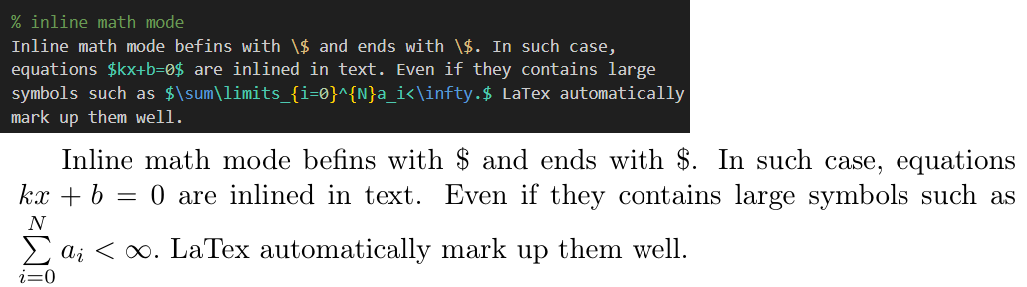
\includegraphics[width=\textwidth]{images/inline_math.png}
    \caption{Inline окружение}
    \label{fig:inline_math}
  \end{figure}

Далее смотрим на displayed окружение. Теория по применению этого типа оружения и примеры верстки приведены на рисунке \ref{fig:displayed_math}.

  \begin{figure}[H]
    \centering
    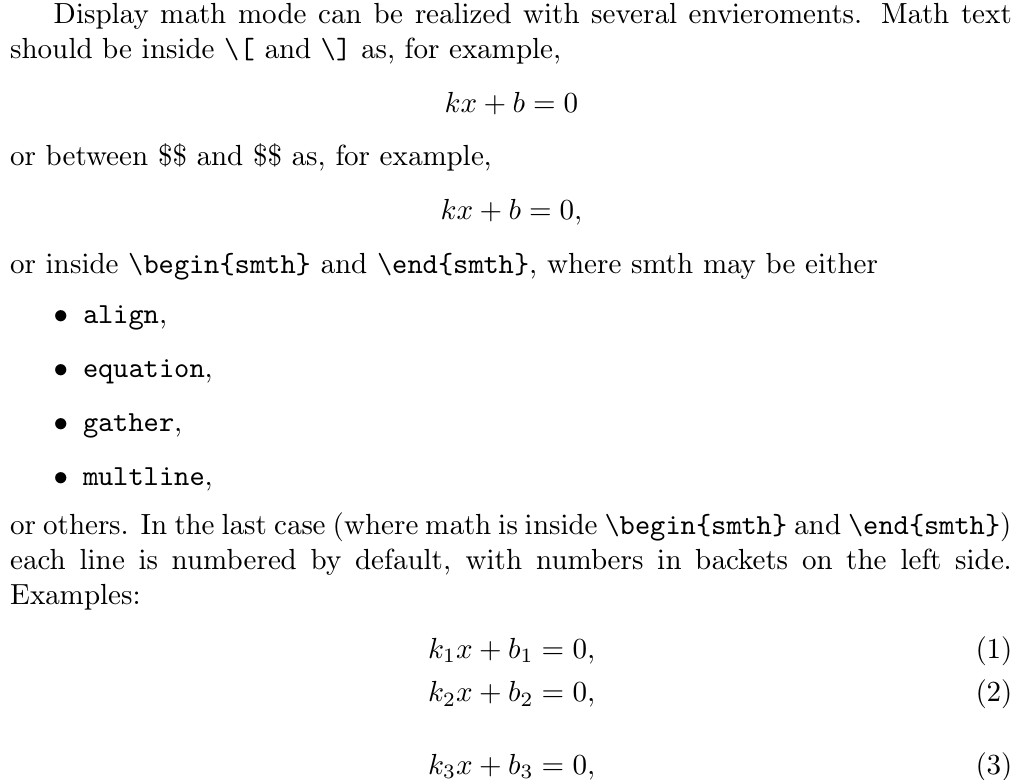
\includegraphics[width=\textwidth]{images/displayed_math.png}
    \caption{Displayed окружение}
    \label{fig:displayed_math}
  \end{figure}

Следующим шагом тестируем ряд изменений шрифта, доступный внутри математического окружения (см. Рис. \ref{fig:math_fonts}).

\begin{figure}[H]
  \centering
  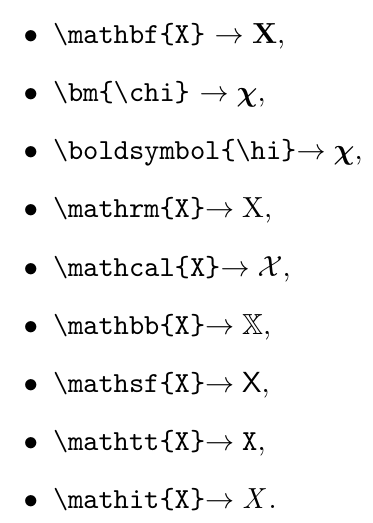
\includegraphics[width=0.5\textwidth]{images/math_fonts.png}
  \caption{Шрифты внутри математического окружения}
  \label{fig:math_fonts}
\end{figure}

Далее испытываем некоторые специальные команды внутри окружения \verb|align|, позволющей разивать уравнения по горизонтали с помощью символов выравнивания \&. Также протестируем грееские символы и принудительное пекращение нумерации уравнений (см. Рис. \ref{fig:special_symbols})

\begin{figure}[H]
  \centering
  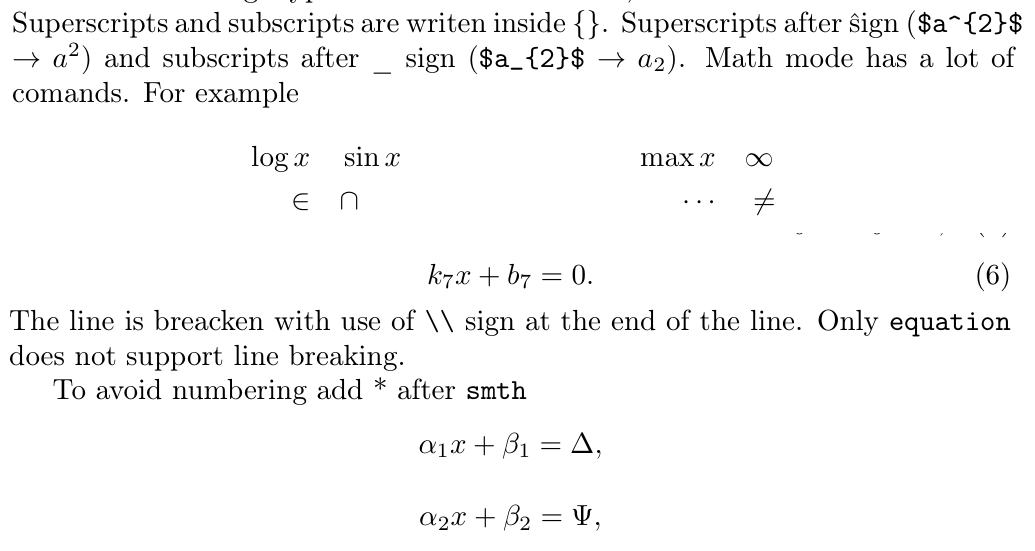
\includegraphics[width=\textwidth]{images/special_symbols.png}
  \caption{Специальные команды, греческий алфавит, приудительная остановка нумерации уравнений, горизонтальное выравнивание с помощью \&.}
  \label{fig:special_symbols}
\end{figure}

Наконец протестируем опции \verb|fleqn| и \verb|leqno|, используемые в команде \verb|\documentclass|, например следующим образом \verb|\documentclass[fleqn]{article}|. Первая опция используется для автоматического выравнивания уравнений по левой стороне. Вторая опция используется для автоматического расположения номеров уравнений слева страницы. Результаты компиляции документов с данными опциями приведены на рисункх  \ref{fig:left_aligment} и \ref{fig:left_numbers}.

\begin{figure}[H]
  \centering
  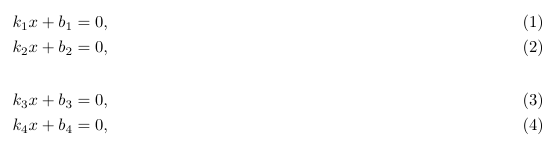
\includegraphics[width=\textwidth]{images/left_aligment.png}
  \caption{Результат компиляции документа с опцией  fleqn}
  \label{fig:left_aligment}
\end{figure}

\begin{figure}[H]
  \centering
  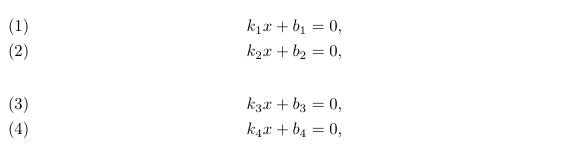
\includegraphics[width=\textwidth]{images/left_numbers.png}
  \caption{Результат компиляции документа с опцией leqno}
  \label{fig:left_numbers}
\end{figure}

\section{Выводы}

В данной работе я освоила работу с математическими окружениями в LaTex, позволяющими верстать профессионально оформленные математические тексты, без затруднений использовать специальные символы и дополнительные шрифты. Я изучила основы синтаксиса и протестировала несколько различных математических окружений. Дополнительно провела эксперимент добавления опций к классу документа, позволяющих изменить выравнивание по умолчанию. 

\bibliography{bib}
\bibliographystyle{IEEEtran}

\end{document}